\itemhead{习题4.2 · 第6题（教材p.113）}{XJ-B1-C04-HW-P113-Y1566}
\label{XJ-B1-C04-HW-P113-Y1566}
{\footnotesize 湘教版教材p.113 / PDF第120页 / 习题4.2 / 第6题}
\field{原题}{在同一平面直角坐标系中画出 $y=4^x$，$y=4^{-x}$，$y=4^{x+1}$，$y=4^{x-1}$ 的图象，并说明后三个函数的图象分别可以由第一个函数的图象怎样变换得到。}
\field{参考答案}{后三图依次由 $4^x$ 关于 $y$ 轴对称、向左平移1、向右平移1得到；可各取三点 $x=-1,0,1$ 求值画图，均保持正函数值。}
\begin{center}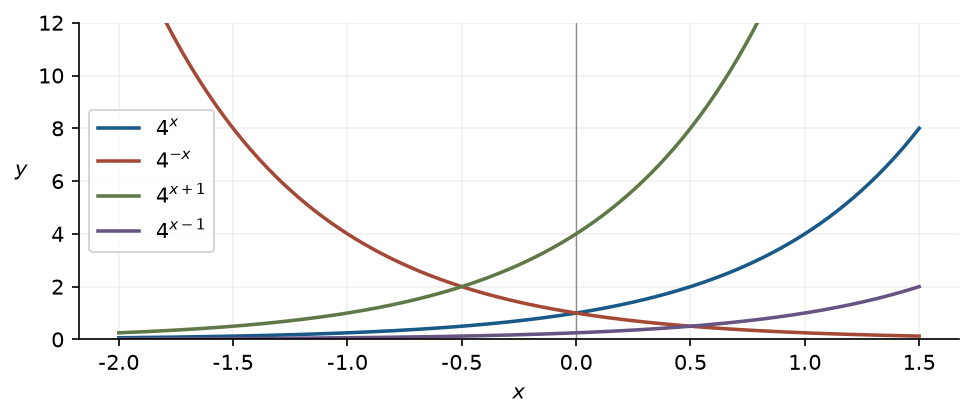
\includegraphics[width=.84\linewidth,height=.38\textheight,keepaspectratio]{figures/C04-HW113-6.png}\end{center}
{\small \field{关联知识}{F09 图象平移、伸缩与对称（教材帮p.86、94 / PDF95、103）；E01 指数函数的概念、图象与性质（教材帮p.150、151 / PDF159、160）}
\field{方法与易错点}{追踪点 $(u,f(u))$ 变换后的坐标，反推新解析式。 易错：平移只改公式而未改定义域；把纵向倍率当作指数底数变化。}
\field{答案依据}{答案册相关题组：PDF第32页（册内页31）；按当前题库原题逐项重算，不按旧版题号机械对套。}}
